% Source for the figure of ConcurrentUnionFind (sec. 24.6): a forest of
% parents before unite(6, 5) and after it, the splitting of find(6) having
% given 6 its grandparent 3 and the root 3 hooked under the root 0. Build:
% make figures (in ../build).
\documentclass[border=4pt]{standalone}
\usepackage[T1]{fontenc}
\usepackage{newpxtext,newpxmath}
\usepackage[varqu,varl,scaled=0.95]{zi4}
\usepackage{tikz}
% tikz-ads.tex: the TikZ styles shared by the figures of the memory of the
% manual, \input by each standalone figure: a cell of a vector (cell), the
% cell that an operation touches (touched), a free cell (free), a node of a
% linked structure (node), the labels of indices (index) and of variables
% (var), a pointer (ptr), and \cells and \indices to draw a row of cells.
\usetikzlibrary{arrows.meta,positioning,calc,fit,shapes.multipart}
\definecolor{adsTouched}{RGB}{214,196,236}
\definecolor{adsFree}{RGB}{236,236,236}
\tikzset{
  ads/.style={>={Stealth[length=2mm]},font=\small,
              every node/.append style={inner sep=0pt}},
  cell/.style={draw,minimum width=7mm,minimum height=7mm,
               font=\small\ttfamily,outer sep=0pt},
  touched/.style={cell,fill=adsTouched},
  free/.style={cell,fill=adsFree,text=black!45},
  node/.style={draw,rounded corners=1pt,minimum width=8mm,
               minimum height=6mm,font=\small\ttfamily},
  index/.style={font=\scriptsize\ttfamily,text=black!60},
  var/.style={font=\small\itshape},
  ptr/.style={->,thick}
}
% \cells{name}{x,y}{list}: a row of cells, the first at (x,y), named
% name-0, name-1, ...; each item is text/style, the style one of cell,
% touched and free (e.g., {a/cell,e/touched,/free})
\newcommand{\cells}[3]{%
  \foreach \v/\s [count=\i from 0] in {#3}
    \node[\s] (#1-\i) at ($(#2)+(\i*7mm,0)$) {\v};}
% \indices{name}{n}: the indices 0 .. n-1 under the cells of name
\newcommand{\indices}[2]{%
  \foreach \i in {0,...,\numexpr#2-1\relax}
    \node[index,below=1.2mm of #1-\i] {\i};}

\begin{document}
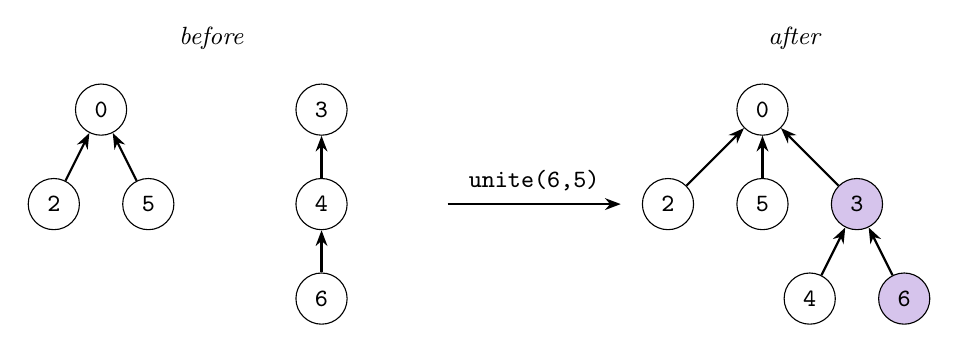
\begin{tikzpicture}[ads,
    el/.style={draw,circle,minimum size=6.5mm,font=\small\ttfamily},
    elt/.style={el,fill=adsTouched}]
  \node[var] at (14mm,9mm) {before};
  \node[el] (a0) at (0,0) {0};
  \node[el] (a2) at (-6mm,-12mm) {2};
  \node[el] (a5) at (6mm,-12mm) {5};
  \node[el] (a3) at (28mm,0) {3};
  \node[el] (a4) at (28mm,-12mm) {4};
  \node[el] (a6) at (28mm,-24mm) {6};
  \draw[ptr] (a2) -- (a0); \draw[ptr] (a5) -- (a0);
  \draw[ptr] (a4) -- (a3); \draw[ptr] (a6) -- (a4);
  \draw[ptr] (44mm,-12mm) -- node[above=1.5mm,font=\small\ttfamily]
    {unite(6,5)} (66mm,-12mm);
  \node[var] at (88mm,9mm) {after};
  \node[el] (b0) at (84mm,0) {0};
  \node[el] (b2) at (72mm,-12mm) {2};
  \node[el] (b5) at (84mm,-12mm) {5};
  \node[elt] (b3) at (96mm,-12mm) {3};
  \node[el] (b4) at (90mm,-24mm) {4};
  \node[elt] (b6) at (102mm,-24mm) {6};
  \draw[ptr] (b2) -- (b0); \draw[ptr] (b5) -- (b0);
  \draw[ptr] (b3) -- (b0); \draw[ptr] (b4) -- (b3); \draw[ptr] (b6) -- (b3);
\end{tikzpicture}
\end{document}
